\section{Training Details}
The Residual TRAIN view partitions into 1,055 verified-correction windows, 311,945 causal teacher-BC windows, and 176,888 stable-identity windows. These sum to 489,888. Parent classes can overlap; the union has 1,917 distinct parent origins. The Risk view has 3,163 nominal TRAIN parents and 695,381 windows. Validation remains fixed at eight nominal parents, with seven admitted Residual parents.

Risk training draws 5\% recovery-associated and 95\% background samples with parent balancing. Residual sampling first chooses BC/identity/recovery at masses 0.2/0.4/0.4 and then selects an origin, branch, and window. Each epoch draws 32,768 samples with replacement. Repeated window draws contribute optimizer updates rather than additional independent scene origins.

The Risk and Residual AdamW weight decays are 0.02 and 0.01. Dropout is 0.20 and 0.10, gradient clipping is 1.0, the maximum epoch budget is 60, and early-stopping patience is 12. Risk is retained at epoch 7 of 19; Residual is retained at epoch 33 of 45. The matching Risk checkpoint is frozen throughout Residual training.

For correction and BC, $\mathcal{L}=0.8\mathcal{L}_{\mathrm{first}}+0.2\mathcal{L}_{\mathrm{horizon}}$, with horizon weights $[4,3,2,1,1,1,1,1]$. Identity penalizes requested arm offsets and smoothness penalizes adjacent horizon differences under the respective availability masks. The raw target contract is an absolute requested offset before limiting, rather than an increment to the previous effective offset.

Tracking uses masked MSE. Required-contact loss refers to opposing right-hand contact during lift/hold; it is not a generic contact-occupancy target. Contact, balance, intervention, and future-onset labels use valid-label BCE. Onset labels exclude current violations and verified-recovery windows. Causal teacher-BC states do not supply nominal Risk labels.

\begin{figure*}[t]
\centering
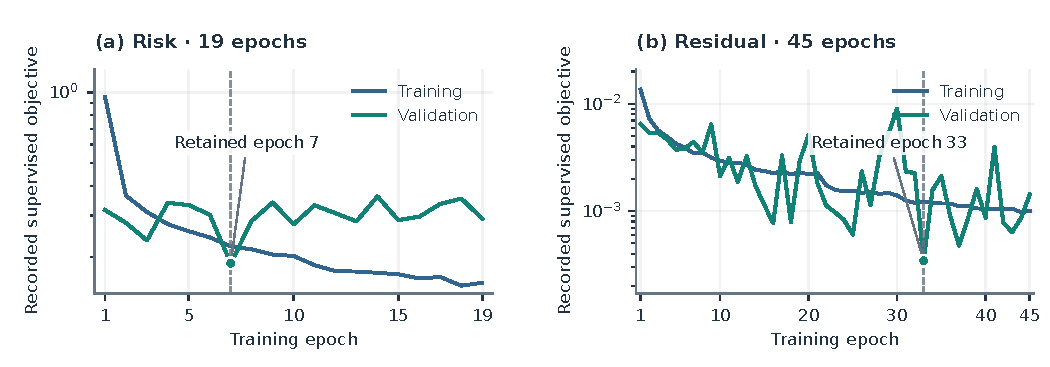
\includegraphics[width=\textwidth]{figures/learning-curves.pdf}
\caption{Recorded optimization histories for the reported controller. Retained checkpoints follow validation objectives, while task improvement is evaluated separately in actual simulated execution.}
\end{figure*}

\section{Complete Confirmation Accounting}
The primary cohort schedules origins $76912+4i$, $i=0,\ldots,127$, prospectively. Origins 76992, 77144, 77304, and 77416 have common nominal-anchor rejection; both scored arms remain unattempted. Origin 77256 has a candidate operational failure and is unsuccessful in the end-to-end endpoint; baseline also fails there. The primary 124 pairs give 49 shared successes, 45 shared failures, 25 rescues, and five harms. The strict completed-physical subset has 123 pairs and 54 baseline versus 74 corrected successes, provided descriptively without an additional test.

The complete-pair effect is $(25-5)/124=16.129\%$. The exact two-sided paired test uses the saved prospective allocation $\alpha=0.00625$ within a maximum-eight comparison family. The nominal 95\% paired-origin percentile interval uses 100,000 resamples and RNG seed 261010. With four unresolved pairs among 128 scheduled origins, the empirical all-origin effect bounds are $(20-4)/128$ to $(20+4)/128$, or $[12.50,18.75]$ percentage points. These bounds describe missing outcomes and are not confidence intervals.

Both branches share cached references where requests are covered. An uncovered phase or duration is generated natively from that branch's current state under the same frozen rule. Treatment order alternates by the original origin index. This symmetric hybrid protocol allows feedback-dependent generation; it does not assert that all branches execute one identical fixed reference sequence. There are no replacement origins, repeated failed physical attempts, or outcome-dependent cohort extensions.

\section{Invocation Ablation and Timing Scope}
The separate same-weight cohort has 20 scheduled origins and 60 scored arms. Two origins, 78196 and 78216, have native lower-replan joint-range guard failure in both learned arms. All four failures remain unsuccessful end-to-end. The strict completed-physical subset has 18 origins and successes 3/18, 10/18, and 14/18 for baseline, selective, and always-on. The primary descriptive ablation table uses all 20 origins, yielding 3/20, 10/20, and 14/20.

Selective has 4,172 Risk decisions and 1,575 Residual invocations; always-on has 4,075 of each. Mean Risk inference is 2.290 versus 2.265\,ms; mean active Residual inference is 1.727 versus 1.713\,ms. Controller means include preparation and both learned components when invoked. Pooled decisions arise on each branch's own trajectory and are not independent task trials or a full-system throughput measurement.

\section{Artifact and Video Guide}
The \href{https://github.com/Peneplain/dl/tree/main/docs/report/videos}{public video supplement} identifies successful and failed trials for both generators and the learned extension. Each clip links text instructions to stages, simulation time, and robot behavior. Its public manifest records scene IDs, camera views, terminal outcomes, file sizes, and SHA-256 hashes. The manuscript names the methods ARDY baseline, Kimodo baseline, and Ours.

The \href{https://github.com/Peneplain/dl/tree/main/docs/report/results}{public result summaries} cover the generator benchmark, controller confirmation, training histories, invocation ablation, and efficiency measurements, with hashes identifying their source records. Editable figures and scripts accompany the \href{https://github.com/Peneplain/dl/tree/main/docs/report}{report source}. Video frames come from saved states; the contact evaluator operates at 200\,Hz, so rendered 50\,Hz frames illustrate behavior without replaying every evaluated contact event.

\section{Generator Benchmark Details}
The two generator batches use the same requests and seeds 60000--60099. All 100 paired scene hashes and SONIC manifests match. The shared scene draws block XY positions from $[0.36,0.46]\times[-0.30,-0.16]$\,m, uses direct standing start and 0.2\,m table standoff, open-hand approach, two automatic 1.6\,s alignment replans, 0.3\,s acquisition transition, 4.8\,s lift, and 5\,s final hold. Finger PD gains are $K_P=6$, $K_D=0.4$. Kimodo retains wrist offset $(0.125,0.035,0.080)$\,m; ARDY uses the measured hand-center default. These adapter settings ground the common grasp goal in each model's interface.

\begin{table}[t]
\centering
\caption{Terminal failure categories}
\begin{tabular}{lrr}
\toprule
Terminal reason & ARDY & Kimodo\\
\midrule
Alignment missed & 0 & 28\\
Grasp not acquired & 17 & 4\\
Timeout & 18 & 9\\
Loss after success threshold & 16 & 3\\
Prohibited robot--table contact & 6 & 0\\
Prohibited robot--block contact & 1 & 0\\
Block--floor contact & 0 & 1\\
Lower/lift execution error & 2 & 0\\
\midrule
Total unsuccessful & 60 & 45\\
\bottomrule
\end{tabular}
\end{table}
Each unsuccessful trial contributes one recorded terminal reason. The \href{https://github.com/Peneplain/dl/tree/main/docs/report/results}{published benchmark summary} gives the terminal counts, paired outcomes, scene/SONIC agreements, and source-record hashes. Command-response time includes grounding, generation, and transition setup; it is not isolated model-forward latency. Native generation rates of 25\,Hz and 30\,Hz describe the sampled motion, not response throughput.

\begin{figure}[t]
\centering
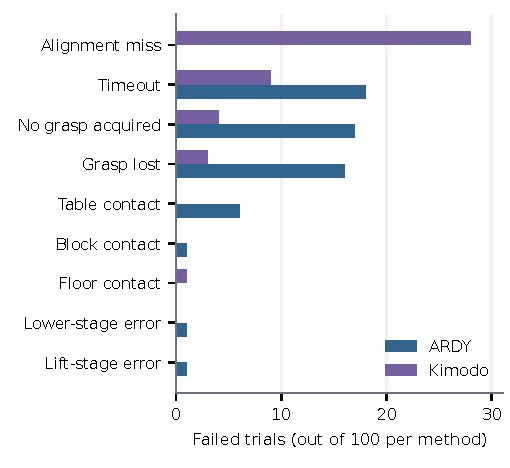
\includegraphics[width=\columnwidth]{figures/failure-profile-column.pdf}
\caption{Recorded terminal failure categories for the shared 100-origin generator benchmark. Counts include every unsuccessful scheduled trial.}
\end{figure}

\section{Paired Execution Examples}
\begin{figure*}[t]
\centering
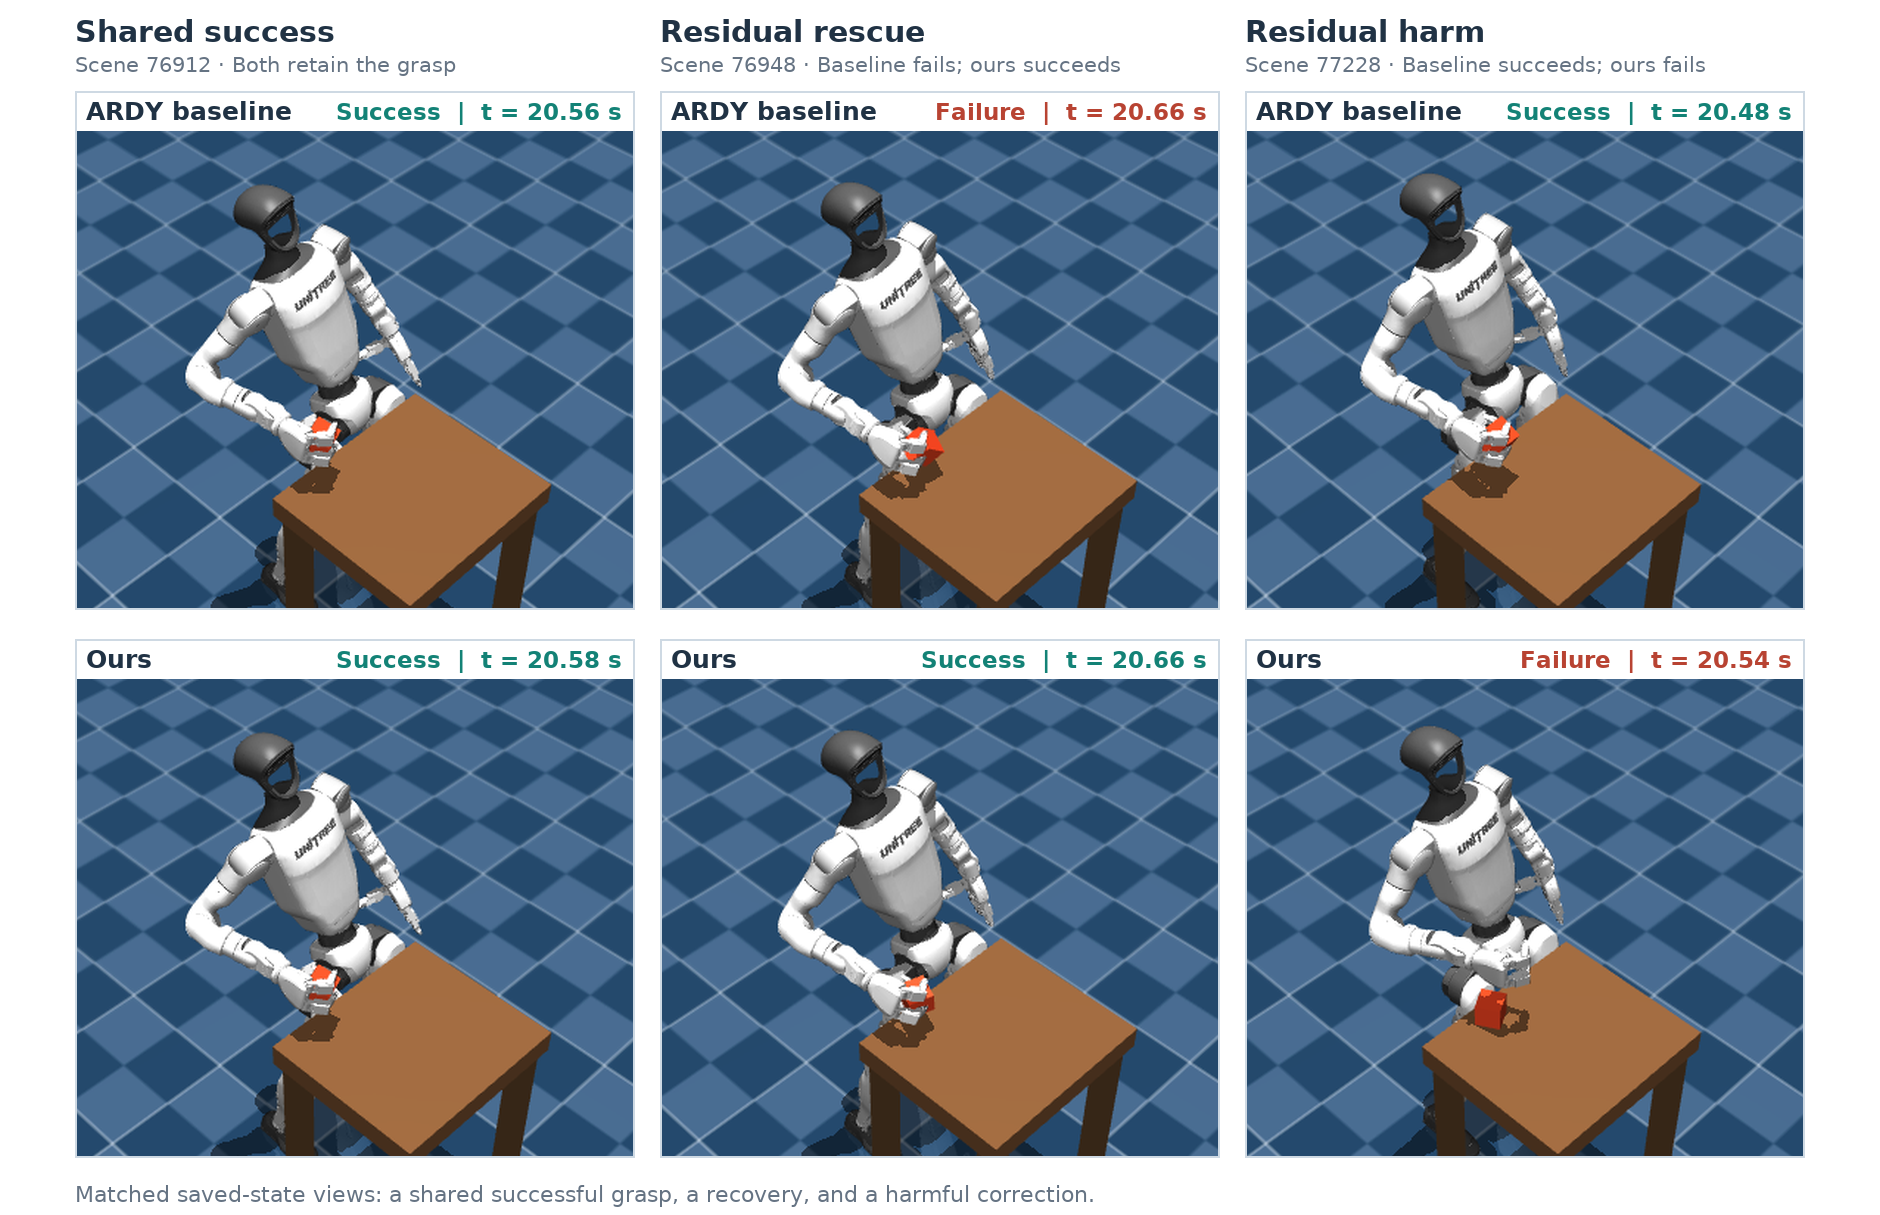
\includegraphics[width=0.88\textwidth]{figures/qualitative.png}
\caption{Paired final states from the independent learned-controller cohort. Columns show shared success, recovery, and harmful correction; rows show ARDY baseline and Ours. The accompanying videos show the preceding contact, lift, and retention sequence.}
\label{fig:qualitative}
\end{figure*}
